% Literature Review
\glsresetall

This chapter delves deeper into the current \gls{sota} and the 
foundational work that has contributed to its development. 
It is divided into sections covering the foundational elements 
of reinforcement learning, the evolution to multi-agent systems, 
and the progression to heterogeneous-agent systems. 
The chapter will conclude by examining some of the open questions, 
unaddressed challenges, and potential future directions in the field.

% ------------------------------------------------------------------------------
\section{Reinforcement Learning Foundations}%

    \subsection*{Markov Decision Processes}%

\Glspl{mdp} form the foundation of reinforcement learning by providing 
a formal framework for modeling decision-making in environments with 
stochastic dynamics~\cite{puterman2005}. An MDP is defined by a tuple 
(\gls{S}, \gls{A}, \gls{P}, \gls{R}, \gls{discount}), where:
\begin{itemize}
    \item \gls{S} is a finite set of states.
    \item \gls{A} is a finite set of actions.
    \item \(\gls{P}: S\times A\times S\rightarrow [0,1]\) is the state 
        transition probability function, where \(P(s^\prime|s, a)\) 
        represents the probability of transitioning to state \(s^\prime\in S\)
        given the current state \(s\in S\) and action \(a\in A\).
        This captures the stochastic nature of the environment.
    \item \(\gls{R}: S \times A \rightarrow \gls{reals}\) is the reward 
        function and written as \(R(s, a)\) defines the immediate reward 
        received after taking action \(a\in A\) in state \(s\in S\). 
        This reward guides the agent's learning process.
    \item \(\gls{discount} \in [0, 1]\) is the discount factor, which 
        determines the level of importance given to estimated future rewards. 
        Specifically, \(\gls{discount}=1\) implies that a reward estimate is 
        given equal value regardless of how many steps in the future it may 
        be while \(\gls{discount}=0\) implies that only the value of a 
        reward in the next step is considered.
\end{itemize}

\begin{figure}
    \centering
    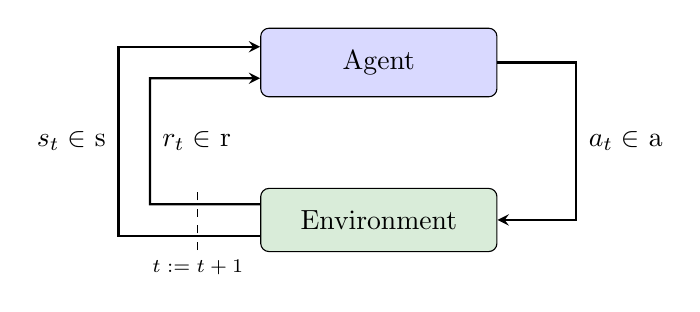
\begin{tikzpicture}[>=stealth, node distance=1cm, on grid, auto,
    entry/.style = {draw, rectangle, inner sep=8pt, rounded corners=3pt,
                    minimum width=3cm},
    arrow/.style = {thick,-stealth}]

    % States
    \node [] (center) {};
    \node [entry, fill= Blue!15] (agent) [above=of center] {Agent};
    \node [entry, fill=Green!15] (env) [below=of center] {Environment};
    \node [] (time) [below left= 0.6cm and 2.3cm of env]{\scriptsize\(t:=t+1\)};
    \draw [dashed] (time) -- +(0,1);

    % Transitions
    \draw [arrow] (agent.east) -- +(1,0) --coordinate(A) +(1,-2) -- (env.east);
    \draw [arrow] ([yshift=-0.2cm]env.west) -- +(-1.8,0) --coordinate(S) 
                    +(-1.8,2.4) -- ([yshift=+0.2cm]agent.west);
    \draw [arrow] ([yshift=+0.2cm]env.west) -- +(-1.4,0) --coordinate(R) 
                    +(-1.4,1.6) -- ([yshift=-0.2cm]agent.west);

    % Labels
    \node [] () [right= 1pt of A] {\(a_t\in\) \Gls{a}};
    \node [] () [left=  1pt of S] {\(s_t\in\) \Gls{s}};
    \node [] () [right= 1pt of R] {\(r_t\in\) \Gls{r}};
\end{tikzpicture}
    \caption{Fully reduced \glsentryshort{mdp} 
        representation of \glsentryshort{rl}.}
    \label{fig:mdp_cycle}
\end{figure}

    \subsection*{Objectives in MDPs}%

The objective in an \gls{mdp} is to find a policy 
\(\gls{pi}: \gls{S} \rightarrow \gls{A}\) that maximizes a return value. 
In the context of an episode it may be referred to as expected cumulative 
reward or \gls{etdr}, and in the context of a single time-step, 
the return \gls{G_t} at time \(t\) is defined as the sum of discounted rewards:
\begin{equation}
    \gls{G_t} = \sum_{k=0}^{\infty} \gls{discount}^k \gls{R}_{t+k+1}
    \label{eq:sum_discounted_rewards}
\end{equation}
where \(\gls{R}_{t+k+1}\) is the reward received following time step \(t+k\).
At the simplest level, reward is translated into a policy using either a 
value function; which may be a state-value or an action-value function 
(\cref{eq:state-value_function,eq:action-value_function} respectively).
A state-value function \gls{v_pi(s)} represents the expected return starting 
from state \(s\) and following policy \gls{pi}. It is generally defined as:
\begin{equation}
    \gls{v_pi(s)} 
    = \mathbb{E}_\pi [\gls{G_t}| \gls{S}_t = s] = \mathbb{E}_\pi \left[
        \sum_{k=0}^{\infty} \gls{discount}^k \gls{R}_{t+k+1} 
        \middle| \gls{S}_t = s \right]
    \label{eq:state-value_function}
\end{equation}
The action-value function \gls{q_pi(a|s)} represents the expected return 
starting from state \(s\), taking action \(a\), 
and thereafter following policy \gls{pi}:
\begin{equation}
    \gls{q_pi(a|s)} 
    = \mathbb{E}_\pi [\gls{G_t}| \gls{S}_t = s, \gls{A}_t = a] 
    = \mathbb{E}_\pi \left[ 
        \sum_{k=0}^{\infty} \gls{discount}^k \gls{R}_{t+k+1}
        \middle| \gls{S}_t=s, \gls{A}_t=a \right]
    \label{eq:action-value_function}
\end{equation}

    \subsection*{Bellman Equations and Optimal Policies}%

The Bellman equations provide recursive definitions for the value functions. 
\Cref{eq:bellman_state-value,eq:bellman_action-value} are the Bellman equations
of the state-value and action-value functions for a given policy \gls{pi} 
respectively.
\begin{equation}
    \gls{v_pi(s)} 
    = \sum_{a \in \gls{A}} \gls{pi}(a|s) 
      \sum_{s^\prime \in \gls{S}} \gls{P}(s^\prime|s, a) \left[
        \gls{R}(s, a) + \gls{discount} v_\pi(s^\prime)\right]
    \label{eq:bellman_state-value}
\end{equation} \begin{equation}
    \gls{q_pi(a|s)} 
    = \sum_{s^\prime \in \gls{S}} \gls{P}(s^\prime|s, a) \left[
        \gls{R}(s, a) + \gls{discount} \sum_{a^\prime \in \gls{A}} 
        \gls{pi}(a^\prime|s^\prime) q_\pi(s^\prime, a^\prime)\right]
    \label{eq:bellman_action-value} 
    \vspace*{1em}
\end{equation}
The goal is to find (or approximate) the optimal policy \gls{pi} that maximizes
the value functions for all states. The optimal Bellman equations are those that
satisfy \cref*{eq:bellman_optimal_state-value,eq:bellman_optimal_action-value}:
\begin{equation}
    \gls{v_*(s)} = \max_a \sum_{s^\prime \in \gls{S}} \gls{P}(s^\prime|s, a)
    [\gls{R}(s, a) + \gls{discount} v_*(s^\prime)]
    \label{eq:bellman_optimal_state-value}
\end{equation} \begin{equation}
    \gls{q_*(a|s)} = \sum_{s^\prime \in \gls{S}} \gls{P}(s^\prime|s, a) 
    [\gls{R}(s, a) + \gls{discount} \max_{a^\prime} q_*(s^\prime, a^\prime)]
    \label{eq:bellman_optimal_action-value}
\end{equation}

    \subsection*{Solution Methods}%

There are numerous methods for solving \glspl{mdp}, including exact methods 
like value iteration and policy iteration, as well as approximate methods 
such as \gls{rl} techniques. Exact methods iteratively compute the value 
functions and improve the policy until convergence to the optimal solution. 
However, for large state and action spaces, 
these methods become computationally infeasible.

In contrast, \gls{rl} methods, which develop policies through interaction
with the environment, offer a scalable approach for solving problems that
can be modelled as \glspl{mdp}. 
\Gls{rl} methods do not require a model of the environment's dynamics and can
handle large, complex problems where exact methods are intractable.
Before examining \gls{rl} approaches to multi-agent systems, we will cover 
several important concepts from the perspective of a single agent system.

% ------------------------------------------------------------------------------
\section{Single-Agent Reinforcement Learning}%

Single-agent \gls{rl} extends the foundational principles of \glspl{mdp} 
by enabling an agent to learn optimal policies through direct interaction with 
the environment. In single-agent \gls{rl}, the agent learns by trial and error, 
using feedback in the form of rewards to adjust its actions and maximize 
cumulative rewards over time.
Single-agent \gls{rl} employs various algorithms to learn the optimal policy by 
approximating the value functions. These algorithms can be broadly categorized 
into dynamic programming, Monte Carlo methods, and \gls{td} learning~%
\cite{sutton2018}.

    \subsection*{Dynamic Programming}%

Dynamic programming methods, such as value iteration and policy iteration, 
require a complete model of the environment's dynamics~\cite{sutton2018}.
They iteratively update value functions and policies until convergence. 
\textbf{Value Iteration} updates the value function based on the Bellman 
optimality equation until it converges to the optimal value function \(v_*\).
\textbf{Policy Iteration} alternates between policy evaluation 
(computing the value function for a fixed policy) and policy improvement 
(improving the policy based on the current value function) until convergence.

    \subsection*{Monte Carlo Methods}%

Monte Carlo methods learn directly from an agent's experience in an episode, 
estimating value functions by averaging the returns observed in actual episodes.
These methods are model-free and do not require knowledge of the environment's 
dynamics. They are generally divided into two categories; 
\textbf{First-Visit Monte Carlo}, averaging the returns of the first visit to 
each state, or \textbf{Every-Visit Monte Carlo}, averaging the returns of every
visit to each state in a given episode.
%
\begin{wrapfigure}[7]{R}{0.4\textwidth}
    \vspace*{-4em}
    \centering
    \resizebox{0.3\textwidth}{!}{%
        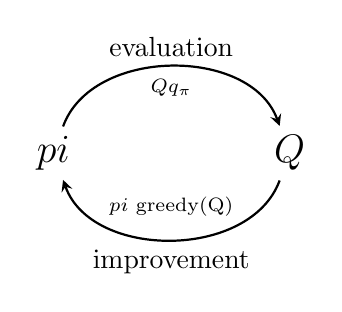
\begin{tikzpicture}[>=stealth, node distance=1.5cm, on grid, auto,
    arrow/.style = {thick,-stealth}]

    % States
    \node [] (center) {};
    \node [] (policy) [left=of center ] {\Large \(\gls{pi}\)};
    \node [] (values) [right=of center] {\Large \(\gls{Q}\)};

    % Transitions
    \draw [arrow] (policy) edge[bend left=70] node(E) {evaluation} (values);
    \draw [arrow] (values) edge[bend left=70] node(I) {improvement} (policy);
    \node [] () [below=15pt of E] {\scriptsize\(\gls{Q}\rightsquigarrow q_\pi\)};
    \node [] () [above=20pt of I] {\scriptsize\(\gls{pi}\rightsquigarrow\) 
        greedy(\gls{Q})};
\end{tikzpicture}
    }
    \captionsetup{margin=1.2em}
    \caption{Generalized Policy Iteration.}
    \label{fig:gpi_cycle}
\end{wrapfigure}
%
In either method, the policy and action values are updated iteratively.
Sutton and Barto~\cite{sutton2018} provide a graphic intuition for this 
iterative cycle, which we have replicated in~\cref{fig:gpi_cycle}.

A key distinction between Monte Carlo in this context and methods described 
later is that Monte Carlo methods execute an entire episode. In the following 
section, this principle will be applied to smaller segments of experience. 
Additionally, we will reference \gls{mcts}, 
a heuristic that simulates the results of future actions. Despite its name, 
\gls{mcts} is distinct from the Monte Carlo methods discussed here.

    \subsection*{Temporal-Difference (TD) Learning}%

\Gls{td} learning methods, such as Q-learning and SARSA 
(State-Action-Reward-State-Action), combine ideas from 
dynamic programming and Monte Carlo methods. They update value estimates 
based on observed transitions without waiting for the end of an episode.
Both methods use an \gls{step-size} parameter to determine the size of 
the update based on \cref{eq:action-value_function}.

\textbf{SARSA} is an on-policy \gls{td} control algorithm that updates the 
\gls{Q}-value using the \gls{Q}-value of the actual next state-action pair:
%
\begin{equation}
    \gls{Q}(s, a) \leftarrow \gls{Q}(s, a) + \gls{step-size} \left[ 
        \gls{R} + \gls{discount} \gls{Q}(s^\prime, a^\prime) - \gls{Q}(s, a) 
    \right]
    \label{eq:sarsa_action-value}
\end{equation}
%
\textbf{Q-Learning}~\cite{watkins1992} is an off-policy \gls{td} control 
algorithm that updates the \gls{Q}-value using the maximum \gls{Q}-value of 
from all actions available to the next state:
%
\begin{equation}
    \gls{Q}(s, a) \leftarrow \gls{Q}(s, a) + \gls{step-size} \left[ 
        \gls{R} + \gls{discount} \max_{a^\prime} 
        \gls{Q}(s^\prime, a^\prime) - \gls{Q}(s, a)
    \right]
    \label{eq:q-learning_action-value}
\end{equation}
%
Consequently, Q-learning has a tendency to converge faster than SARSA,
which may or may not be a desirable feature.

    \subsection*{Exploration vs. Exploitation}

A fundamental challenge in \gls{rl}, as it is in all of machine learning, 
is balancing exploration (trying new actions to discover their effects) 
and exploitation (choosing actions known to yield high rewards). 
Common strategies for addressing this balance include \(\epsilon\)-greedy 
policies and Boltzmann exploration.
\(\epsilon\)-greedy increases the exploration of an algorithm by selecting
a random action \(\epsilon\) percent of the time.
%
Boltzmann exploration, commonly using a softmax function~\cite{pan2021}, 
normalizes estimated action-values to reduce bias during action selection. 
A temperature parameter \(\tau\) may be included to control the exploration 
rate over time, similar to a simulated annealing heuristic. 
%\Cref{eq:softmax_action-value} shows an example of this.
For example,
%
\begin{equation}
    P(A=a|S=s) =
    \frac{\exp\left\{\gls{Q}(a|s)/\tau\right\}}{
        \sum_{a^\prime\in A}\exp\left\{\gls{Q}(a^\prime|s)/\tau\right\}}
    \label{eq:softmax_action-value}
\end{equation}
However, \cite{cesa-bianchi2017} argue that this manner of 
implementation fails to minimize regret compared to \(\epsilon\)-greedy 
and attribute it to the difficulty in tuning a \(\tau\) decay schedule~
\cite{kaelbling1996,vermorel2005}.

% ------------------------------------------------------------------------------
\section{Evolution to Multi-Agent Systems}%

The evolution from single-agent \gls{rl} to multi-agent systems introduces new 
complexities and opportunities, reflecting more realistic scenarios where 
multiple agents interact within a shared environment. \Gls{marl} extends the 
principles of single-agent RL to settings where agents must learn to 
cooperate, compete, or coexist, each influencing the other's learning process.
Key developments in centralized and decentralized training, communication and 
coordination, scalability, and stability have significantly expanded the 
applicability of \gls{marl} across various domains. 

    \subsection*{Cooperative and Competitive Multi-Agent Systems}%

In cooperative multi-agent systems, agents work together to achieve a 
common goal. This requires coordination and communication to ensure that 
their actions complement each other. Cooperative MARL is often applied 
in tasks where the joint effort of multiple agents can lead to better 
performance than individual efforts~\cite{littman1994}.

The primary challenge in cooperative \gls{marl} is to develop 
strategies that maximize the collective reward~\cite{albrecht2024}. 
This involves a spectrum of approaches to the level of interaction 
between agents. Here we focus on interactions at the algorithmic level, 
rather than within the environment. On one end, 
a set of agents may be trained and deployed in a fully decentralized
manner~\cite{li2023d} and on the other,
we have integration such that the agents are simply copies of each other,
updating a shared policy~\cite{zheng2017}.

Rather than emphasizing either extreme, the majority of research in \gls{marl} 
has focused on leveraging interactions to produce more effective results. 
The most popular approaches fall under the label \gls{ctde}~%
\cite{foerster2017,rashid2018,fotouhi2019,lowe2020,pan2021,%
papoudakis2021,li2023d,zhou2023}, 
%
\begin{wrapfigure}[9]{R}{0.4\textwidth}
    \vspace*{-2.5em}
    \centering
    %\includegraphics[width=0.3\textwidth]{basic_ctde.png}
    %\resizebox{0.3\textwidth}{!}{%
        \documentclass{standalone}
\usepackage[dvipsnames]{xcolor}
\usepackage{tikz}
\usetikzlibrary{positioning, shapes, arrows,}

\begin{document}
\colorlet{DarkGreen}{Black!25!Green}
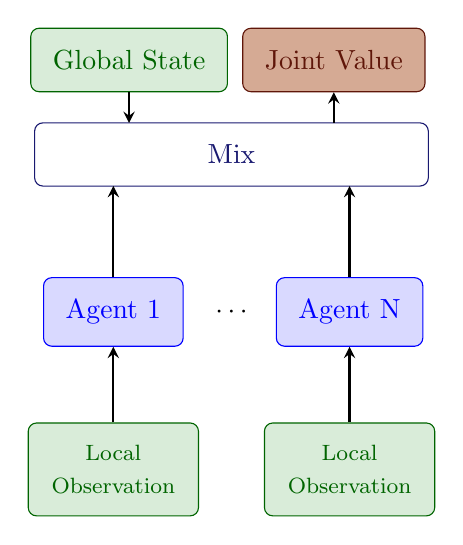
\begin{tikzpicture}[>=stealth, node distance=2cm, on grid, auto,
    entry/.style = {draw, rectangle, inner sep=8pt, rounded corners=3pt,
                    minimum width=1.5cm},
    greenEntry/.style = {draw, rectangle, inner sep=8pt, rounded corners=3pt,
                minimum width=1.5cm, align=center, DarkGreen, fill=Green!15},
    blueEntry/.style = {draw, rectangle, inner sep=8pt, rounded corners=3pt,
                    minimum width=1.5cm, Blue, fill=Blue!15},
    arrow/.style = {thick,-stealth}]

    % Entries
    \node [] (center) {\(\cdots\)};
    \node [blueEntry] (agent_1) [left =1.5cm of center] {Agent 1\ };
    \node [blueEntry] (agent_n) [right=1.5cm of center] {Agent N};
    \node [entry, MidnightBlue] (mix) [above=of center, minimum width=5cm] {Mix};
    \node [greenEntry] (state) [above left=1.2cm and 1.3cm of mix] 
        {Global State};
    \node [entry, Sepia, fill=Sepia!25] (value) [above right=1.2cm and 1.3cm of mix] {Joint Value};
    \node [greenEntry, text width=1.6cm] (obs_1) [below=of agent_1] 
        {\footnotesize Local Observation};
    \node [greenEntry, text width=1.6cm] (obs_n) [below=of agent_n] 
        {\footnotesize Local Observation};

    % Relations
    \draw [arrow] (obs_1) -- (agent_1);
    \draw [arrow] (obs_n) -- (agent_n);
    \draw [arrow] (agent_1) -- +(0,1.6);
    \draw [arrow] (agent_n) -- +(0,1.6);
    \draw [arrow] (state) -- +(0,-0.8);
    \draw [arrow] (value)+(0,-0.8) -- (value) ;
\end{tikzpicture}


\end{document}
    %}
    %\captionsetup{margin=1.2em}
    \caption{Basic \gls{ctde}.}
    \label{fig:basic_ctde}
\end{wrapfigure}
%
a broad term encompassing any algorithm with an arbitrary centralizing 
mechanism. We assert that the term's breadth and ubiquity have made it 
a defining trait of mainstream \gls{marl} and that it will remain the 
norm until we begin to examine \gls{harl} algorithms.

Within the \gls{ctde} paradigm, we wish to draw particular attention to 
actor-critic training, derived from an almost identical single-agent 
training method. It is an intuitive implementation of \gls{ctde}, 
where the critic performs the role of mixing for the agents. 
The majority of the algorithms we will examine in our experiments 
will either be actor-critic~\cite{foerster2017,lowe2020,li2023c} 
or will aim to reduce the bias that occurs with a singular, 
shared critic~\cite{rashid2018,ackermann2019,li2023d,zhou2023}.






%%%%%%%%%%%%%%%%%%%%%%%%%%%%%%%%%%%%%%%%%%%%%%%%%%%%%%%%%%%%%%%%%%%%%%%%%%%%%%%%
% --------------------------------- Edit Bar --------------------------------- %
%%%%%%%%%%%%%%%%%%%%%%%%%%%%%%%%%%%%%%%%%%%%%%%%%%%%%%%%%%%%%%%%%%%%%%%%%%%%%%%%








In competitive multi-agent systems, agents have conflicting goals. 
The success of one agent typically comes at the expense of another,
and thus are often modeled as zero-sum games, where the 
gain of one agent is exactly balanced by the loss of another.

Thus competitive \gls{marl} typically involves strategies where agents 
must predict and counteract the actions of their opponents. 
Techniques from game theory, such as Nash equilibrium, are often employed 
to find stable strategies in these adversarial environments~\cite{busoniu2008}.



%\subsubsection*{Communication and Coordination}
Effective communication and coordination mechanisms are crucial for cooperative \gls{marl}. 
Agents need to share information and synchronize their actions to achieve common goals. 
Research in this area focuses on developing protocols and algorithms that enable efficient and 
robust communication among agents~\cite{sukhbaatar2016,fotouhi2019,hoang2023}.

%\subsubsection*{Scalability and Efficiency}
Scalability is a significant challenge in MARL due to the exponential growth of the state and 
action spaces with the number of agents\cite{cao2012,busoniu2008}. 
Recent research efforts aim to develop algorithms that can efficiently scale to large numbers 
of agents and complex environments without compromising performance~\cite{smit2023,sun2023}.

%\subsubsection*{Stability and Convergence}
Ensuring the stability and convergence of learning algorithms in multi-agent settings is 
critical~\cite{papoudakis2021}. 
Unlike single-agent \gls{rl}, where convergence is well-understood, 
the dynamics of multiple learning agents can lead to instability and non-convergence.
Research in this area seeks to establish theoretical guarantees and practical methods 
for stable learning.

% ------------------------------------------------------------------------------
\section{Evolution of MARL through the Lens of Games}%

Building upon these foundational advancements, the exploration of 
\gls{marl} through gameplay has provided a rich and challenging testbed for further innovation. 
Notably, the strategic complexity and real-time decision-making required in games have driven 
remarkable progress in \gls{marl} algorithms, as exemplified by pioneering projects such as 
DeepMind's AlphaGo\cite{silver2016}, AlphaGo Zero\cite{silver2017},
AlphaZero\cite{silver2017a} and AlphaStar\cite{vinyals2019}. 
These projects not only showcase the potential of \gls{marl} to achieve superhuman performance 
but also highlight the broader implications and applications of these advancements 
beyond the realm of gaming.

\subsection*{AlphaGo: The First* Milestone}
AlphaGo, developed by DeepMind and presented in~\cite{silver2016}, 
marked perhaps the largest milestone in \gls{ai} since Deep Blue~\cite{campbell2002}
with its victory over a world champion Go player.
Where Deep Blue was an expert system that leveraged an Alpha-Beta pruning algorithm
and \glspl{asic} designed to execute the algorithm in parallel,
the state-space of Go was so much larger that this approach would not likely ever be tractable. 
AlphaGo achieved this success using \glspl{dnn} to approximating a value function and a policy.

An initial approximate policy was trained on 29.4 million states from 160,000 games
using supervised gradient descent to predict the next move of a game given the current state.
An initial value function was approximated by sampling moves made during a game
and assigning value according to the outcome of the game.

With initial approximate functions as a starting point,
a policy-gradient method in conjunction with \gls{mcts}
would provide the the framework for further improvement through \gls{rl}.

\subsection*{AlphaGo Zero: A Leap Forward}
AlphaGo's success demonstrated the power of combining deep learning with traditional 
search techniques. However, the research team acknowledged potential problems associated with 
the original approach's reliance on prepared data. 
In~\cite{silver2017}, Silver et al. express a concern regarding 
possible expense, unreliability, or unavailability of relevant data for pre-training.
They developed a new approach to address these concerns and titled it AlphaGo Zero.
Here we focus on two key factors that made this possible.

First, the employment of the \gls{dnn} was simplified by combining the value function and policy 
into a single network that would take a state input and return a vector of move probabilities and 
a state value, this substantially reduced the cost of updating the network(s) during training.




Second,
training using self-play.




The transition from 






\begin{comment}
AlphaGo Zero’s Innovation
AlphaGo Zero represented a significant leap forward by eliminating the need for human expert knowledge. Unlike its predecessor, AlphaGo Zero learned to play Go entirely from self-play, starting with random moves and improving solely through reinforcement learning.
	•	Key Techniques:
	•	Self-Play Learning: AlphaGo Zero trained by playing games against itself, using a single neural network that combined the policy and value functions.
	•	Simplified Architecture: The simplified neural network architecture and reliance on self-play allowed for more efficient training and faster improvement.
	•	Key Paper: Silver, D. et al. (2017). Mastering the game of Go without human knowledge.
Impact
AlphaGo Zero’s success underscored the potential of self-play and reinforcement learning to achieve superhuman performance without human intervention. This approach demonstrated the scalability and generality of MARL techniques, opening new possibilities for their application in other domains.

AlphaStar: Expanding to Real-Time Strategy Games
AlphaStar’s Achievement
AlphaStar extended the principles of MARL to the domain of real-time strategy (RTS) games by achieving grandmaster-level performance in StarCraft II, a game known for its strategic depth, real-time decision-making, and partial observability.

	•	Key Techniques:
	•	Multi-Agent Learning: AlphaStar was trained using a league of agents that played against each other, promoting diverse strategies and robust learning.
	•	Imitation and Reinforcement Learning: AlphaStar initially used imitation learning from human expert games, followed by reinforcement learning through self-play to refine its strategies.
	•	Modular Neural Network Architecture: The architecture included components for managing different aspects of the game, such as strategy, tactics, and unit control.
	•	Key Paper: Vinyals, O. et al. (2019). Grandmaster level in StarCraft II using multi-agent reinforcement learning.

Broader Implications

AlphaStar’s success highlighted the adaptability of MARL to more complex, dynamic, and partially observable environments. The techniques developed for AlphaStar are applicable to a wide range of real-world problems, such as autonomous vehicle coordination, resource management, and robotic control.

Additional Achievements and Related Developments

OpenAI Five

OpenAI’s Dota 2 project, OpenAI Five, further showcased the capabilities of MARL in complex, team-based, real-time strategy games. By training a team of agents to play against top human players, OpenAI demonstrated the potential for AI to handle teamwork, strategy, and adaptation in highly dynamic environments.

	•	Key Techniques:
	•	Self-Play and Reinforcement Learning: Similar to AlphaStar, OpenAI Five used extensive self-play and reinforcement learning to develop sophisticated strategies.
	•	Curriculum Learning: The training process involved progressively increasing the difficulty of opponents to ensure continuous improvement.
	•	Key Paper: Berner, C. et al. (2019). Dota 2 with Large Scale Deep Reinforcement Learning.

Summary

The evolution of MARL through the lens of game-playing AI demonstrates the transformative impact of reinforcement learning and self-play on achieving superhuman performance in complex environments. The successes of AlphaGo, AlphaGo Zero, AlphaStar, and OpenAI Five illustrate the potential for MARL to tackle a wide range of strategic and real-time challenges, paving the way for future advancements in both theoretical research and practical applications.

	•	Key Papers:
	•	Silver, D. et al. (2016). Mastering the game of Go with deep neural networks and tree search.
	•	Silver, D. et al. (2017). Mastering the game of Go without human knowledge.
	•	Vinyals, O. et al. (2019). Grandmaster level in StarCraft II using multi-agent reinforcement learning.
	•	Berner, C. et al. (2019). Dota 2 with Large Scale Deep Reinforcement Learning.




%\subsection*{Applications of MARL}
%\Gls{marl}has been applied to a wide range of domains, 
%demonstrating its versatility and effectiveness in solving complex, real-world problems. 
%Notable applications include:
    3.3 Applications of MARL
	•	Autonomous Driving: Coordinated control of multiple autonomous vehicles to improve traffic flow and safety.
	•	Robotics: Multi-robot systems for tasks such as search and rescue, where robots must collaborate to achieve a common objective.
	•	Economics and Finance: Modeling and simulation of market dynamics involving multiple agents with competing interests.
	•	Healthcare: Optimizing the allocation of resources and coordination of treatments across multiple healthcare providers.
	•	Key Paper: Yang, Y. et al. (2023). Efficient policy learning in large-scale heterogeneous-agent environments.
    3.2 Advances in MARL
    The advancement of MARL includes the development of algorithms that allow agents to learn in environments with other learning agents, leading to applications in fields such as robotics, game theory, and economics.
        •	Key Paper: Busoniu, L., Babuska, R., & De Schutter, B. (2008). A comprehensive survey of multi-agent reinforcement learning.
        •	Key Paper: Mnih, V. et al. (2015). Human-level control through deep reinforcement learning.
        •	Key Paper: Silver, D. et al. (2017). Mastering the game of Go without human knowledge.
\end{comment}


\section{Introduction to Heterogeneous-Agent Reinforcement Learning}





\clearpage
\begin{comment}
    4. HARL
    HARL extends MARL by allowing agents with different capabilities and knowledge to interact. 
    This heterogeneity mirrors real-world scenarios more closely, where agents (e.g., robots, drones) often have diverse functionalities.
4.1 Definition and Significance
	•	Key Paper: Lowe, R. et al. (2017). Multi-Agent Actor-Critic for Mixed Cooperative-Competitive Environments.
4.2 Applications of HARL
HARL has been applied in various domains such as autonomous driving, smart grids, and collaborative robotics, demonstrating its potential to solve complex, real-world problems.
	•	Key Paper: Kraemer, L., & Banerjee, B. (2020). Multi-agent reinforcement learning as a rehearsal for decentralized planning.
5. \section{Current State of the Art in HARL}
5.1 Recent Advances
Recent research has focused on enhancing the efficiency, scalability, and robustness of HARL algorithms. Significant contributions include the development of new learning paradigms and the application of HARL in increasingly complex environments.
	•	Key Paper: Zhou, Y. et al. (2023). The role of hierarchy in multi-agent learning.
	•	Key Paper: Yang, Y. et al. (2023). Efficient policy learning in large-scale heterogeneous-agent environments.
5.2 Addressing Strategic Collapse
One critical challenge in HARL is the risk of strategic collapse, where agents’ strategies become suboptimal when scaling up the number of agents or increasing environmental complexity. Addressing this issue is crucial for the practical deployment of HARL systems.
	•	Key Paper: Papoudakis, G. et al. (2021). Benchmarking Multi-Agent Deep Reinforcement Learning Algorithms.
	•	Key Paper: Foerster, J. et al. (2018). Learning with Opponent-Learning Awareness.
6. Open Challenges and Future Directions
6.1 Scalability and Efficiency
Improving the scalability and computational efficiency of HARL algorithms remains a significant challenge. Research in this area focuses on optimizing algorithms to handle large-scale agent populations without sacrificing performance.
	•	Key Paper: Baker, B. et al. (2020). Emergent Tool Use from Multi-Agent Autocurricula.
6.2 Policy Generalization
Ensuring that HARL policies generalize well across different environments and agent configurations is essential for real-world applications. This involves developing robust learning strategies that can adapt to varying conditions.
	•	Key Paper: Shao, K. et al. (2020). Is Multi-Agent Deep Reinforcement Learning the Answer or the Question? A Brief Survey.
7. Conclusion
The field of HARL holds great promise for advancing multi-agent systems, offering solutions to complex problems through the interaction of diverse agents. However, significant challenges remain, particularly in addressing strategic collapse and ensuring scalability and policy generalization. Future research must continue to push the boundaries of HARL, focusing on these critical issues to unlock its full potential.


\section{Multi-Agent Reinforcement Learning}
\subsection*{Multi-Agent Advantage Decomposition}
\subsection*{Simultaneous Update}
\subsection*{Sequential Update}
\section{Heterogeneous-Agent Reinforcement Learning}
\section{Self-play}
\section{Strategic Collapse}
\section{Key Algorithms}
\subsection*{Multi-Agent DQNs}
\subsection*{Actor-Critic methods} % (lowe2020)
\subsection*{Counterfactual Regret Minimization }
\subsection*{Joint Action Learners}
\subsection*{MAPPO}
\subsection*{HAPPO}


%Additionally, mediated reinforcement learning introduces the concept of mediators to ensure 
%cooperation among self-interested agents, promoting socially beneficial behaviors 
%(Ivanov \& Zisman, 2023).

%Techniques like asymmetric-evolution 
%training have been developed to train agents in asymmetrical multiplayer games, showcasing the 
%capability to handle complex interactions and achieve high performance without human data 
%(Sun et al., 2023).

\cite*{zhong2024} for HARL

\end{comment}
\begin{comment}
We intend to use this section for accomplish three things;
\begin{enumerate}
    \item Convince the committee that this is important
    \item Convince the committee that this is an open question
    \item Convince the committee that we understand the current state of the literature and the 
    scope of the intended research. (Implicitly indicating the feasibility of the research)
\end{enumerate}

Include a lit review table.
\begin{tabular}{ccc}
    Paper & contributions & ref 
\end{tabular}
\end{comment}